\documentclass[12pt,a4paper]{report}
\usepackage[utf8]{inputenc}
\usepackage[portuguese]{babel}
\usepackage[T1]{fontenc}
\usepackage{amsmath}
\usepackage{amsfonts}
\usepackage{amssymb}
\usepackage{graphicx}
\usepackage{fourier}
\usepackage{hyperref}
\usepackage{tcolorbox}
\usepackage{qrcode}
\usepackage{fancyhdr}
\pagestyle{fancy}
\lhead{Luiz Guilherme}
\rhead{Professor de Matemática}
\usepackage{fontawesome}
\usepackage{enumerate}
\usepackage[Glenn]{fncychap}

\usepackage[left=2cm,right=2cm,top=2cm,bottom=2cm]{geometry}
\author{Professor LG}
\title{Matemática e Raciocínio Lógico para Concursos}


\newcommand{\questao}[4]
{\begin{tcolorbox} {\textbf{#1}}
{#2} 

 \end{tcolorbox} \\ 
 \begin{minipage}{12cm}   
 \begin{enumerate}   
 	[a)]{#3} 
 \end{enumerate}  
 \end{minipage} 
 \qrcode{#4&list=UULFeA_dOOqAA4DB92B_BWDU7Q} \\
 \vspace{3mm}
 \hline
  \newpage}
\begin{document}

\maketitle
\tableofcontents
\chapter{VUNESP}
\section{Oficial de Justiça 2023}
\questao{Média Aritmética}{O gráfico apresenta o número de acertos na prova de Língua Portuguesa e de Matemática, aplicada a dois candidatos, A e B, em um concurso interno para promoção de cargo:\\
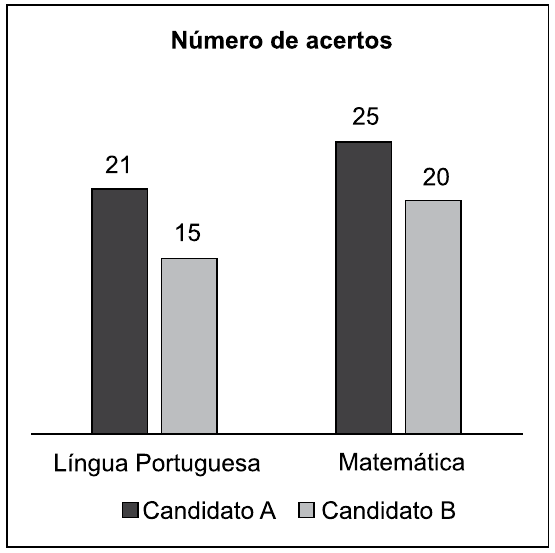
\includegraphics[scale=.5]{fig001.png}\\
Sabendo-se que a prova de Língua Portuguesa tinha peso 2 e a de Matemática tinha peso 3 para o cargo em concurso, que cada uma das provas tinha 50 questões, e que a nota de cada prova é igual ao número de acertos correspondente, é correto afirmar que o número de questões de Matemática que o candidato B deveria ter acertado a mais, para que a média aritmética ponderada das notas das suas provas fosse igual à média aritmética ponderada das notas das provas do candidato A, é igual a}
{
\item 9.
\item 20.
\item 10.
\item 29.
\item 27.}{https://www.youtube.com/watch?v=hcdlzi_qYfc}

\questao{Aritmética Modular}{ Uma empresa executa serviços aos seus clientes somente de segunda-feira a sexta-feira, independentemente de haver feriado ou não. Para seu cliente X&W, ela executa serviços a cada 12 dias, excluindo-se sábados e domingos, enquanto que para seu cliente W&Z, ela executa serviços a cada 33 dias, também excluindo-se sábados e domingos. No dia 15 de agosto de 2023, uma terça-feira, essa empresa executou serviços para ambos os clientes. Isso significa que a vez imediatamente posterior em que ela executou os serviços para ambos os clientes, em um mesmo dia, foi uma}
{
\item sexta-feira.
\item segunda-feira.
\item quinta-feira.
\item quarta-feira.
\item terça-feira.}
{https://www.youtube.com/watch?v=hcdlzi_qYfc}

\questao{Média Aritmética, Razão e Proporção}
{No ano de 2022, 3 em cada 8 edifícios comercializados em determinada região foram adquiridos pelo empreen­dimento A&B, que investiu R\$ 1,35 bilhão na compra desses edifícios, ao preço médio de R\$ 15 milhões cada edifício. Dos edifícios não adquiridos pelo empreendimento A&B e que foram comercializados naquela r­egião, o empreendimento R&T adquiriu metade, ao custo total R\$ 1,23 bilhão, o que fez com que o preço médio, por edifício adquirido pela R&T, fosse de}
{\item R\$ 16,3 milhões.
\item R\$ 16,1 milhões.
\item R\$ 16,5 milhões.
\item R\$ 16,4 milhões.
\item R\$ 16,2 milhões.}
{https://www.youtube.com/watch?v=hcdlzi_qYfc}


\questao{}
{Considere as informações apresentadas na tabela a seguir, relacionadas à produção de certa peça que é
realizada apenas por máquinas iguais, trabalhando ao mesmo tempo, com a mesma capacidade de produção.\\
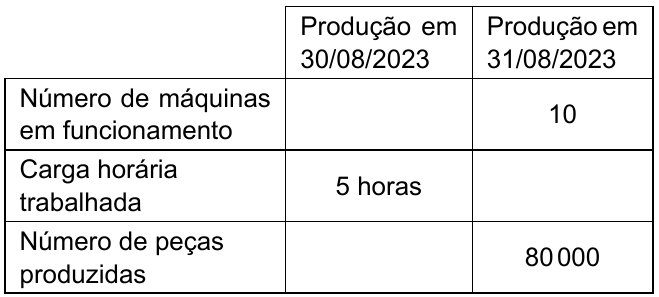
\includegraphics[scale=.5]{fig002}\\
Sabendo-se que as informações apresentadas são proporcionais, que em 30/08/2023 o número de máquinas em funcionamento era um quinto maior que o número de máquinas trabalhando no dia seguinte, e que o número de peças produzidas em 31/08/2023 foi quatro terços do número de peças produzidas no dia anterior, é correto afirmar que a carga horária trabalhada no dia 31/08/2023 foi de}
{
\item 8 horas.
\item 7 horas.
\item 9 horas.
\item 8 horas e 30 minutos.
\item 7 horas e 30 minutos.}
{https://www.youtube.com/watch?v=hcdlzi_qYfc}

\questao{}
{Sabendo-se que é falsidade a afirmação “Se Nora trabalhou, então ela precisa descansar”, assinale a alternativa que apresenta uma afirmação verdadeira.
}
{
\item Nora trabalhou e ela não precisa descansar.
\item Nora não trabalhou e ela não precisa descansar.
\item Nora trabalhou e ela precisa descansar.
\item Nora não trabalhou ou ela precisa descansar.
\item Nora não trabalhou e ela precisa descansar.}
{https://www.youtube.com/watch?v=hcdlzi_qYfc}

\questao{}
{Considere verdadeiras as seguintes premissas:
\begin{enumerate}[I.]
\item Se Carla não é casada ou Pedro não é divorciado, então Cláudio é filho único.
\item Se Sônia é mãe, então Carla não é casada.
\item Se Pedro não é divorciado, então Sergio não é administrador e Gerson é noivo.
\item Cláudio não é filho único.
\end{enumerate}
Uma conclusão que decorre das premissas apresentadas e forma, juntamente com as premissas, um argumento
válido é}
{
\item Gerson é noivo.
\item Sergio não é administrador.
\item Sônia não é mãe.
\item Sônia é mãe.
\item Sergio é administrador.}
{https://www.youtube.com/watch?v=hcdlzi_qYfc}

\questao{}{Sobre um grupo de atletas sabe-se que 15 praticam natação, atletismo e ciclismo, 20 praticam somente n­atação e atletismo, 27 praticam somente natação e c­iclismo, e 25 praticam somente atletismo e ciclismo.\\
Se 70 atletas desse grupo praticam natação, 61 praticam atletismo, e 75 praticam ciclismo, então é verdade que, das alternativas a seguir, a que contém a porcentagem que mais se aproxima da relação entre o número de atletas que praticam um único esporte o número total de atletas desse grupo é
}
{
\item 12\%
\item 18\%
\item 20\%
\item 16\%
\item 14\%}
{https://www.youtube.com/watch?v=hcdlzi_qYfc}

\questao{}
{Na sequência numérica 1, 4, 7, 8, 11,14, 19, 22, 25, 26, 29, 32, 37, ..., o 1º elemento é o número 1. Mantida a regularidade, o 11 111º elemento é o número}
{
\item 33 332.
\item 31 111.
\item 33 115.
\item 33 329.
\item 32 228.}
{https://www.youtube.com/watch?v=hcdlzi_qYfc}

\questao{}
{Considere a seguinte afirmação: “Ou durmo ou trabalho”. Uma negação lógica para a afirmação apresentada é}
{
\item Ou não durmo ou não trabalho.
\item Trabalho ou durmo.
\item Se não durmo, então não trabalho.
\item Não trabalho e não durmo.
\item Durmo se, e somente se, trabalho.}
{https://www.youtube.com/watch?v=hcdlzi_qYfc}

\questao{}
{Considere verdadeira a afirmação “Se Marcelo é professor universitário, então Raquel é advogada” e falsa a afirmação “Marcelo é professor universitário e Raquel é advogada”.\\
Nessas condições, é necessariamente verdade que}
{
\item Marcelo não é professor universitário.
\item Raquel não é advogada.
\item Marcelo é professor universitário.
\item Marcelo é professor universitário ou Raquel não é advogada.
\item Raquel é advogada.}
{https://www.youtube.com/watch?v=hcdlzi_qYfc}








\end{document}